\documentclass[tikz,border=8pt]{standalone}
% Shared look for every TikZ diagram. Load with \input{../../tools/tikz-style.tex}
\usepackage[sfdefault]{roboto}
\usetikzlibrary{arrows.meta, positioning, shapes.geometric, calc, fit, backgrounds}
\definecolor{cblue}{HTML}{4C78A8}
\definecolor{corange}{HTML}{F58518}
\definecolor{cgreen}{HTML}{54A24B}
\definecolor{cred}{HTML}{E45756}
\definecolor{cpurple}{HTML}{B279A2}
\definecolor{cgrey}{HTML}{6B6B6B}
\tikzset{
  every picture/.style={font=\sffamily, line width=1.2pt},
  box/.style={draw=#1, fill=#1!12, rounded corners=4pt, align=center, inner sep=7pt, minimum height=1.1cm},
  box/.default=cgrey,
  arrow/.style={-{Stealth[length=3mm]}, draw=cgrey, line width=1.4pt},
  title/.style={font=\sffamily\bfseries\Large},
  note/.style={font=\sffamily\small, text=cgrey, align=center},
}
\AtBeginDocument{\hyphenpenalty=10000 \exhyphenpenalty=10000}

% Why the speed settles and the heading swings: from what the motors set to what we control, the speed is one
% adding-up away from the force, the heading two adding-ups away from the torque. Numbers from headkit.py.
\begin{document}
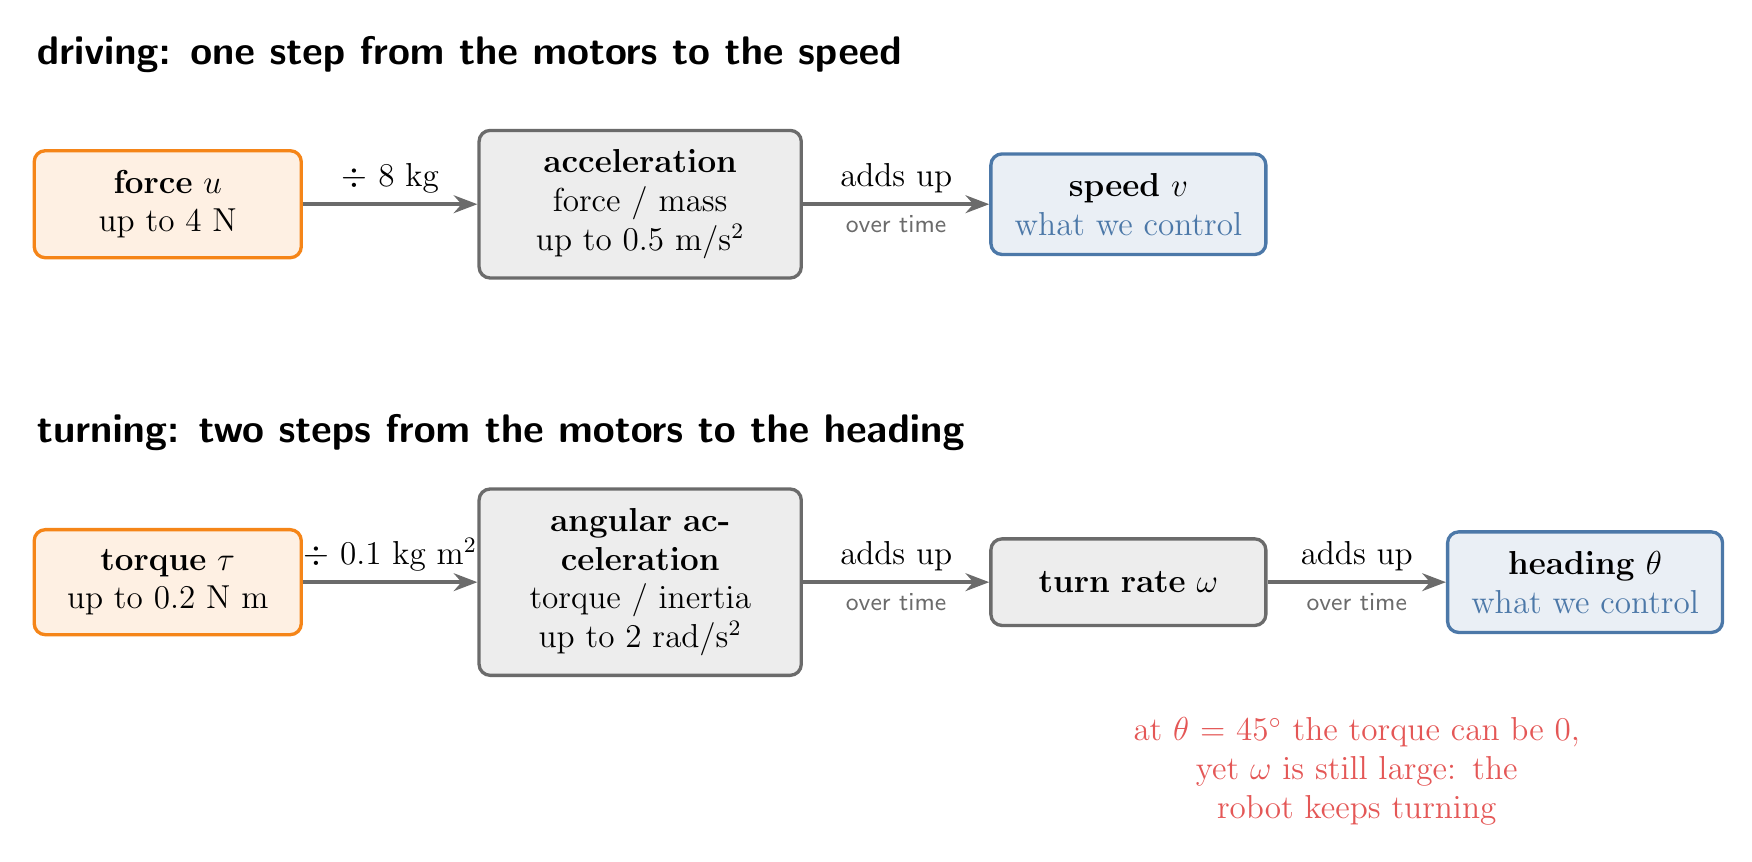
\begin{tikzpicture}[every node/.append style={font=\large}]
  \node[title, anchor=west] at (-1.4,1.9) {driving: one step from the motors to the speed};
  \node[box=corange, text width=2.9cm] (f) at (0.4,0) {\textbf{force} $u$\\ up to 4 N};
  \node[box=cgrey, text width=3.6cm] (a) at (6.4,0) {\textbf{acceleration}\\ force / mass\\ up to 0.5 m/s$^2$};
  \node[box=cblue, text width=3.0cm] (v) at (12.6,0) {\textbf{speed} $v$\\ \textcolor{cblue}{what we control}};
  \draw[arrow] (f) -- node[above] {$\div$ 8 kg} (a);
  \draw[arrow] (a) -- node[above] {adds up} node[below, note] {over time} (v);

  \node[title, anchor=west] at (-1.4,-2.9) {turning: two steps from the motors to the heading};
  \node[box=corange, text width=2.9cm] (t) at (0.4,-4.8) {\textbf{torque} $\tau$\\ up to 0.2 N m};
  \node[box=cgrey, text width=3.6cm] (al) at (6.4,-4.8) {\textbf{angular acceleration}\\ torque / inertia\\ up to 2 rad/s$^2$};
  \node[box=cgrey, text width=3.0cm] (w) at (12.6,-4.8) {\textbf{turn rate} $\omega$};
  \node[box=cblue, text width=3.0cm] (th) at (18.4,-4.8) {\textbf{heading} $\theta$\\ \textcolor{cblue}{what we control}};
  \draw[arrow] (t) -- node[above] {$\div$ 0.1 kg m$^2$} (al);
  \draw[arrow] (al) -- node[above] {adds up} node[below, note] {over time} (w);
  \draw[arrow] (w) -- node[above] {adds up} node[below, note] {over time} (th);
  \node[note, font=\large, text=cred, text width=6.4cm] at (15.5,-7.2)
     {at $\theta$ = 45$^\circ$ the torque can be 0,\\ yet $\omega$ is still large: the robot keeps turning};
\end{tikzpicture}
\end{document}
